\documentclass{article}

\usepackage{color}
\usepackage{graphicx}
%\usepackage{subfigure}
\usepackage{listings}
\usepackage[OT2,OT1]{fontenc} % Used for in-line transliterated cyrillic
\usepackage{stmaryrd}

\definecolor{red}{rgb}{1,0,0}
\definecolor{red}{rgb}{0,0,1}

\newcommand{\mnote}[1]{\marginpar{%
  \vskip-\baselineskip
  \raggedright\footnotesize
  \itshape\hrule\smallskip\tiny{#1}\par\smallskip\hrule}}  

\newcommand{\todo}[1]{\textcolor{blue}{(#1)}}
\newcommand{\mtodo}[1]{\mnote{\textcolor{red}{#1}}}

\newcommand{\secref}[1]{Section~\ref{#1}}
\newcommand{\tabref}[1]{Table~\ref{#1}}
\newcommand{\figref}[1]{Figure~\ref{#1}}
\newcommand{\lstref}[1]{Listing~\ref{#1}}
\def\bs#1{\boldsymbol{#1}}

\DeclareTextFontCommand{\cyr}{\renewcommand\rmdefault{wncyr}\renewcommand\sfdefault{wncyss}\renewcommand\encodingdefault{OT2}\normalfont\selectfont}
\DeclareTextFontCommand{\cyri}{\renewcommand\rmdefault{wncyr}\renewcommand\sfdefault{wncyss}\renewcommand\encodingdefault{OT2}\normalfont\itshape\selectfont}
\DeclareTextFontCommand{\cyrb}{\renewcommand\rmdefault{wncyr}\renewcommand\sfdefault{wncyss}\renewcommand\encodingdefault{OT2}\normalfont\bfseries\selectfont}

\lstset{ %
%keywordstyle=\color{black}\bfseries\underbar,
keywordstyle=\color{blue}\bfseries\underbar,
language=XML,                % choose the language of the code
basicstyle= \footnotesize\tt,       % the size of the fonts that are used for the code
%numbers=left,                   % where to put the line-numbers
%numberstyle=\tiny\tt,      % the size of the fonts that are used for the line-numbers
%stepnumber=1,                   % the step between two line-numbers. If it's 1 each line  will be numbered
%numbersep=5pt,                  % how far the line-numbers are from the code
backgroundcolor=\color{white},  % choose the background color. You must add \usepackage{color}
showspaces=false,               % show spaces adding particular underscores
showstringspaces=false,         % underline spaces within strings
showtabs=false,                 % show tabs within strings adding particular underscores
frame=single,	                % adds a frame around the code
tabsize=2,	                % sets default tabsize to 2 spaces
captionpos=b,                   % sets the caption-position to bottom
breaklines=true,                % sets automatic line breaking
breakatwhitespace=false,        % sets if automatic breaks should only happen at whitespace
title=\lstname,                 % show the filename of files included with \lstinputlisting; also try caption instead of title
escapeinside={\%*}{*)},         % if you want to add a comment within your code
keywords={corpora, resources, preprocessing, output, experiments}            % if you want to add more keywords to the set
}

%This file has been converted to use LaTeX2e
%\documentstyle[dimacs]{article}
%
% any "\include{...}" statements go here
%

\title{Lexicon Induction for Low-resource Languages}

%the first "thanks" for each author should list the affiliation with DIMACS

%\author{ \\ Dept. of Computer Science \\ 
%  Rutgers University \\ New Brunswick, New Jersey 08903
%\and First Middle Last\thanks{Affiliated Graduate Student Member}\thanks{Other
%grant support or acknowledgements.}  \\ Dept. of Computer Science \\
 % Princeton University \\ Princeton, New Jersey 08544}
%\reportno{2000-01}     %DIMACS number, to be assigned after submission of abstract

\begin{document}
\maketitle

\begin{abstract}

Statistical machine translation relies on the availability of substantial amounts of human translated texts. Such bilingual resources are available for relatively few language pairs, which presents obstacles to applying current statistical translation models to low-resource languages. In this work, we induce bilingual dictionaries from more plentiful monolingual corpora using a diverse set of cues, including: cross-lingual vector space models, the frequencies of words over time, orthographic similarity, etc.  We report the efficacy of these monolingual cues and contrast their performance for a language pair where plentiful bilingual resources are available.  We further evaluate the accuracy of bilingual dictionaries induced between English and a set of low resource languages.  Since our principal objective is to induce wide coverage lexicons, we contrast the performance of our framework on randomly selected source words with an optimistic results obtained on frequent words and typically reported in lexicon induction literature.  Finally, we propose a simple and effective technique for using crowd sourced annotations to incrementally refine the output of our lexicon induction system.%\mtodo{Last sentence doesn't fit too well.}
\end{abstract}

\section{Introduction}

Statistical methods for machine translation continue to push the state of the art in automatic translation. However, they crucially rely on the availability of large numbers of translations aligned across two languages. Generation of these parallel corpora require the efforts of bilingual speakers and are extremely expensive to produce in sufficient quantities to induce a high quality statistical translation system.  As a result, these methods can not be successfully applied to the majority of word's languages and especially to low-resource or less frequently taught languages.  The DARPA BABEL (Bayesian Architecture Begetting Every Language) project aims to address the problem of scarcity of bilingual training data.  In this report, we summarize the progress made in eight and a half months since the start of the project, and outline the next steps we are planning to take.\\

The first objective of the BABEL project is to (a) collect large monolingual datasets for a number of low resource languages and (b) utilize them to build alternative bilingual resources for inducing translation models in the absence of large parallel corpora.  In particular, we posit that cheap to collect monolingual resources contain cues which can be utilized for inducing bilingual lexicons. In this report, we define and exploit a handful of these cues to generate wide coverage dictionaries between English and a large set of low density languages.  Prior work on lexicon induction has attempted to automatically learn bilingual lexicons, either by using monolingual corpora (\cite{Rapp:1999}, \cite{Koehn:2002}, \cite{Schafer:2002}, \cite{Haghighi:2008}) or by exploiting the cross-language evidence of closely related “bridge” languages that have more resources \cite{Mann:2001}.  While this work falls into the former category, our objective is substantially different.  Unlike the bulk of the previous work, our specific aim is to use monolingual cues to induce {\em broad coverage} dictionaries for a large set of low resource languages.  In sum, in this report we summarize the progress toward the first objective of the project, i.e.:

\begin{itemize}
 \item Describe monolingual resources we are continuously collecting.
 \item Define a set of cues which we use to induce bilingual lexicons from those resources.
 \item Propose an evaluation method and show preliminary results on a high resource language pair and ten low resource languages and English.
 \item Propose an effective technique for using crowd sourced annotations to incrementally refine the output of our lexicon induction system.
 \item Briefly describe implementation details of the induction framework.
\end{itemize}

The second goal of the BABEL project is to propose novel translation models to utilize these monolingual resources in the absence of large explicitly aligned bilingual corpora.  In this report, we also describe the ongoing work toward introducing these models.\\

%Statistical methods for machine translation continue to push the state of the art in automatic translation. However, they crucially rely on the availability of large numbers of translations aligned across two languages. Generation of these parallel corpora require the efforts of bilingual speakers and are extremely expensive to produce in sufficient quantities to induce a high quality statistical translation system. As a result, these methods can not be successfully applied to the majority of word's languages and especially to low-resource or less frequently taught languages.  On the other hand, we now have access to large and continuously expanding amounts of monolingual data.  We posit that these resources often contain cues which could be effectively utilized for inducing bilingual resources, and we will explore their use in order to reduce and eventually eliminate the need for explicitly aligned bilingual translations.\mtodo{Wordy and vague.}\\

%In this work, we exploit these monolingual cues to induce bilingual lexicons between English and a large set of low-density languages.  Prior work on lexicon induction has attempted to automatically learn bilingual lexicons, either by using monolingual corpora (\cite{Rapp:1999}, \cite{Koehn:2002}, \cite{Schafer:2002}, \cite{Haghighi:2008} or by exploiting the cross-language evidence of closely related “bridge” languages that have more resources \cite{Mann:2001}.  While this work falls into the former category, our objective is substantially different.  Unlike the bulk of the previous work, our specific aim is to use monolingual cues to induce large and {\em broad coverage} dictionaries for a large set of low density languages.\\

%We begin by introducing a set of monolingual cues and studying their efficacy on a language pair for which plentiful bilingual resources are available.  We then use them to induce bilingual lexicons between English and a set of ten diverse low resource languages.  Finally, we propose a simple and effective technique for using crowd sourced annotations to incrementally refine the output of our lexicon induction system.

%A code framework to:
%Define similarity metric
%Extract a scored/ranked list of candidates
%Aggregate multiple cues
%Deal with morphology: currently, a simple heuristic as a placeholder.
%Implemented for time, context, edit distance, and topic (in progress) 
%Extract / clean / language id / extract temporal information from the ongoing clawled pages repository

%-----------------------------------------------------
\section{Related Work} \label{sect:relwork}

%The literature on translation lexicon induction for low-resource languages falls in to two broad categories: 1) utilizing similarity between languages by choosing a high-resource “bridge” language for translation (\cite{Mann:2001}, \cite{Schafer:2002}) and 2) extracting noisy cues from monolingual corpora and using them to associate words across languages.\\

\cite{Rapp:1999} was the first to propose using context of a given word as a clue to its translation. Given a German word with an unknown translation, its surrounding words were collected and translated into English using a small seed dictionary.  Words with similar context in a monolingual English corpus were then proposed as translation candidates.  The original work employed a relatively large bilingual dictionary containing approximately 16,000 words and tested only on a small collection of 100 manually selected nouns.  Subsequent work has explored Rapp's ideas proposing a variety of alternative similarity metrics, better methods for collecting context, and monolingual cues.  \cite{Koehn:2002} used a larger test set consisting of the 1000 most frequent words from a German-English lexicon. They also incorporated cues such as frequency and orthographic similarity in addition to context. \cite{Schafer:2002} independently proposed using frequency, orthographic similarity and also showed improvements using temporal and word burstiness similarity measures, in addition to context.  \cite{Klementiev:2006b} used phonetic and temporal similarity specifically to discover transliterated terms.  \cite{Haghighi:2008} made use of contextual and orthographic cues for learning a generative model from monolingual corpora and a seed lexicon.  \cite{Garera:2009} proposed a dependency-based context model that incorporates long-range dependencies, variable context sizes, and reordering.  \cite{Mimno:2009}, \cite{Boyd-Graber:2009} exploited to use multilingual topic models to discover translations.\\

We first show that evaluation results on a small set of hand selected words typically reported in previous work can be misleading if the objective is to induce large translation dictionaries.  We then investigate the effectiveness of individual monolingual cues for inducing broad coverage lexicons for a large number of low-density languages. \\

%\begin{itemize}
%\setlength{\parskip}{0pt}
%  \item Context: \cite{Rapp:1995,Rapp:1999,Fung:1998}
%  \item Time: \cite{Schafer:2002,Klementiev:2006b}
%  \item Topics: \cite{Mimno:2009,Boyd-Graber:2009}
%  \item Multiple: \cite{Schafer:2002,Koehn:2000,Haghighi:2008}
%  \item Dependecies: \cite{Garera:2009}
%  \item --- Bridge languages: \cite{Mann:2001}
%  \item Combination Strategies: \cite{Koehn:2002,Klementiev:2006b,Klementiev:2008a}
%  \item Mechanical Turk: Following previous work on posting NLP tasks on MTurk \cite{Snow:2008,CCB:2009}, we use the service to gather annotations for proposed bilingual lexicon entries. 
%  \item Other: \cite{Monz:2005}
%\end{itemize}

%-----------------------------------------------------
\section{Inducing Bilingual Lexicons From Monolingual Cues}\label{sect:cues}

Various linguistic and corpus cues can be informative for relating word translations across a pair of languages.\mtodo{Little technical details, i.e. no metric defs, etc. Add?}  We begin by considering a few of them and explain how they can be used to measure similarity between a source word and a translation candidate.

\subsection{Monolingual cues}

\noindent\emph{Contextual cue.} \cite{Rapp:1999} proposed inducing a translation dictionary from disparate monolingual texts.  They populate a bilingual lexicon by projecting {\it context vectors} across two languages using vector-space semantic models to represent words  \cite{Deerwester:1990}.  The elements in vector-based representations of a word indicate the frequency of its co-occurrence with all other words in the same language.  For instance, the vector representation of ``airplane'' would indicate that it frequently occurs in contexts near the words ``airport'', ``flight'', ``landing,'' ``passengers'', ``pilot'', ``runway'',  etc.  The similarities of words within one language can be measured using the distance between their vectors, with cosine similarity, for instance.  To translate unknown words, \cite{Rapp:1999} suggests building vector space models of two languages.  The elements in an unknown word's vector are {\it projected} into the vector space of the other language using the known translations from a small seed bilingual dictionary.  This sparse projected vector is compared to the vectors for all words in the target language.  The word whose vector is most similar to the projected vector is considered to be the best translation of the unknown word.  This process is illustrated in Figure \ref{fig:contextual}.\\

\begin{figure}
\centerline{\mbox{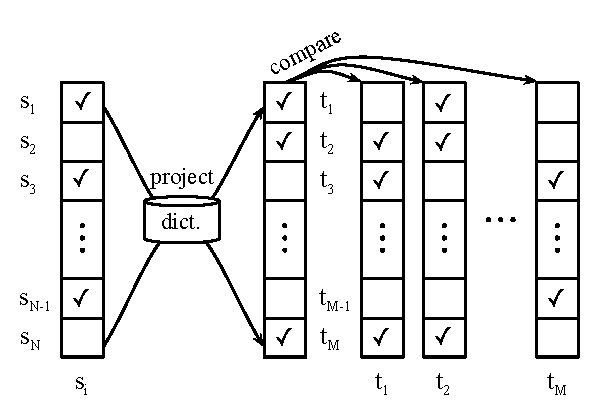
\includegraphics[width=2.8in]{figures/contextual}}}
\caption{Lexicon induction using contextual information. First, contextual vectors are projected using a small seed dictionary and then compared with the target language candidates.}
\label{fig:contextual}
\end{figure}

\noindent\emph{Temporal cue.} Online content is often published along with temporal information: news feeds, for example, are comprised of news stories annotated with date and time of publication.  The feeds are specialized for the target geographical locations and vary in content across languages.  Still, many events are deemed relevant to multiple audiences and the news stories related to them appear in several languages, although rarely as direct translations of one another.  Words associated with these events will appear with increased frequency in multiple languages around the dates when these events are reported.  \figref{fig:temporal} illustrates this idea with temporal histograms of three English words and their Spanish translations. Such weak synchronicity provides a cue about the relatedness of words across the two languages, and can be exploited to associate them.  In order to score a pair of entities across languages, we can compute the similarity of their temporal signatures.\mtodo{\figref{fig:temporal} is from Europarl, add the one from the proposal instead.}\\

\begin{figure}[h]
\centerline{\mbox{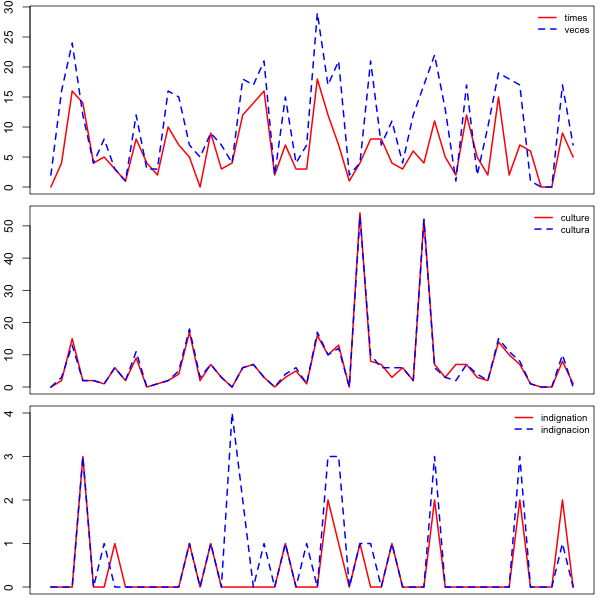
\includegraphics[width=2.8in]{figures/temporal}}}
\caption{Temporal histograms of three English words and their Spanish translations.}
\label{fig:temporal}
\end{figure}

\noindent\emph{Orthographic cue.} Etymologically related words often retain similar spelling across languages with the same writing system.  Capturing these similarities can provide yet another clue about their relatedness.  Edit distance defines one such metric, counting the minimal number of edit operations required to transform one string into another.  While it won't provide a good signal for most translation pairs, it proves to be a highly effective for related languages such as English and Spanish (see \secref{sect:exphigh}). \\

\noindent\emph{Phonetic cue.}  We can extend the previous idea to language pairs not sharing the same writing system, since many cognates and transliterated words are phonetically similar.  \cite{Klementiev:2006b} train a transliteration model to return high scores to phonetically similar word pairs and show it to be highly successful for Named Entities which are often transliterated.  Adding this cue should provide an informative signal for cognates as well. \\

%\noindent\emph{Topic cue.}  Yet another idea is to exploit the category metadata often associated with a piece of text (such as news story or a Wikipedia article), i.e. associate words according to categories they tend to appear in.  

\subsection{Combination Strategies}

These cues provide informative and independent means to score a source word and a target candidate, and combining them is likely to produce better lexicons.  One idea is to directly combine the ranked lists of induced candidates using the mean reciprocal rank (MRR) heuristic frequently used in Information Retrieval literature.  The idea is to score each of the translation candidates with an average reciprocal rank across all rankings, and then sort the candidates in descending order.\\

The relative informativeness of the cues will depend on the data: e.g. the temporal cue depends on the temporal alignment of of both sides of the bilingual corpus, the orthographic cue is uninformative when the two languages use different scripts, etc.  However, the MRR heuristic assigns equal weights to each ranking and investigating more suitable combination strategies remains the subject of ongoing work.\\ 

Some of the metrics we have introduced (e.g. edit distance) are likely to assign same scores to multiple candidates.  We use the following strategy for resolving ties: (1) a set of candidates assigned the same score shares the same rank, (2) a rank assigned to a candidate (a real value) takes into account the number of other candidates with the same or better scores (\figref{fig:rankties}).\\

\begin{figure}
\centerline{\mbox{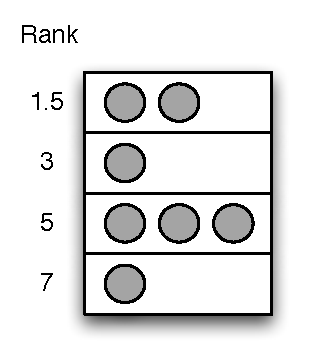
\includegraphics[width=1.3in]{figures/rankties}}}
\caption{Resolving ties.}
\label{fig:rankties}
\end{figure}

\subsection{Handling Morphology} \label{sect:morph}

Many of the languages in our list such as Russian and Korean are characterized by morphological rules generating a large number of word forms for the same lexeme.  Thus, we need to be able to group morphological variants of the same word into an equivalence class and collect their aggregate statistics.  For instance, we would like to count the total number of occurrences of \emph{\{Herzegovina, Hercegovina\}} on the English side in order to map it accurately to the corresponding equivalence class we may see on the Russian side of our corpus (e.g. \cyri{\{Gercegovina, Gercegovinu, Gercegoviny, Gercegovino\U{i}\}}).  In order to keep to our objective of requiring as little language knowledge as possible, we take a rather simplistic approach for grouping equivalence classes.  For morphologically rich languages, a set of words are in the same equivalence class if they share a prefix of size five or longer.  For the other languages, each unique word is assigned its own class.  More sophisticated unsupervised approaches (i.e. \cite{Goldwater:2006}) could be incorporated instead, and are a subject of ongoing work.

%-----------------------------------------------------
\section{Resources} \label{sect:resources}

In this section we briefly describe each of the resources we use for inducing translation lexicons.  For those being continuously collected, we give a current snapshot of relevant statistics.\\

\noindent{\em Wikipedia}. Wikipedia provides a large repository of continuously edited monolingual texts in a large number of languages.  Besides the article content, it also contains various metadata which can be useful for generating additional resources.  For example,
% category information associated with each article can be used induce the topic cue, and 
interlingual links can be used to select articles discussing the same subject across multiple languages.  We will use these comparable articles when inducing translations using the contextual cue in \secref{sect:experiments}.  \tabref{fig:wikidictstats} lists counts of such page pairs between English and 42 other languages along with the second language scripts used predominantly\footnote{While Uzbek, Serbian, Azeri, Kurdish, Kazakh, Uighur, and Somali use multiple writing systems, we indicate only those used for the bulk of Wikipedia articles.} in the corresponding wikis.\\
 
\begin{table}[h!]
\setlength{\tabcolsep}{1ex}
\footnotesize
\begin{center}
\begin{tabular}{l|rrr|rrr|}
\multicolumn{1}{c}{}	&	\multicolumn{3}{c}{Wikipedia}	&	\multicolumn{3}{c}{Dictionary}\\
%\hline
\cline{2-7}% \cline{4-6}
Language	& page pairs	&	trg tokens	&	script	&	entries	&	src type/token	&	script \\
	&	& (thousands)	&	&	&	coverage (\%) &\\
\hline
Tigrinya	&	36	&	3	&	o	&	56	&	0.3/0.6	&	{\bf r}\\
Punjabi 	&	401	&	101	&	o	&	76,311	&	12.2/57.7	&	o/{\bf r}\\ 	
Kyrgyz	&	492	&	77	&	c	&	74,890	&	2.6/42.4	&	{\bf r}\\
Somali 	&	585	&	82	&	r	&	230	&	0.2/6.8	&	r\\ 
Nepali 	&	1,293	&	262	&	d	&	6,812	&	3.6/39.7	&	{\bf r}\\
Tibetan	&	1,358	&	35	&	i	&	59,083	&	2.5/35.1	&	{\bf r}\\
Uighur	&	1,814	&	114	&	a/r	&	16,285	&	1.7/37.9	&	r\\
Maltese 	&	1,896	&	706	&	r	&	7,574	&	2.9/44.7	&	r\\
Turkmen	&	3,137	&	104	&	r	&	91,928	&	4.6/54	&	r\\
Kazakh 	&	3,470	&	606	&	c	&	145,750	&	1/34	&	{\bf r}\\
Mongolian 	&	4,009	&	847	&	c	&	948	&	0.3/20.7	&	{\bf r}\\
Tatar		&	4,180	&	313	&	c/r	&	 8,557	&	1.7/33	&	c/r\\
Kurdish	&	5,059	&	872	&	r	&	9,870	&	1.2/32	&	r\\
Uzbek 	&	5,875	&	747	&	r/c	&	190,688	&	6.2/66.4	&	r\\
Kapampangan	&	6,827	&	875	&	r	&	1,000	&	0.2/7	&	r\\
Urdu 	&	7,674	&	2,163	&	u	&	36,428	&	2.9/57.1	&	{\bf r}\\
Irish	&	9,859	&	2,183	&	r	&	887&	0.2/23.5	&	r\\
Azeri	&	12,568	&	2,518	&	r	&	231,891&	0.6/42.7	&	r\\
Tamil	&	13,470	&	3,484	&	m	&	165,004	&	2.6/43.6	&	m\\
Albanian 	&	13,714	&	3,197	&	r	&	188,563	&	5.4/55.6	&	r\\
Afrikaans	&	14,315	&	4,637	&	r	&	11,389	&	0.8/50.2	&	r\\
Hindi 	&	14,824	&	5,349	&	d	&	58,179	&	2.2/37.7	&	{\bf r}\\
Bangla 	&	16,026	&	2,607	&	b	&	1,606	&	0.2/20.6	&	b/{\bf r}\\
Tagalog	&	17,757	&	2,534	&	r	&	247,662	&	3.5/65.8	&	r\\
Latvian	&	22,737	&	5,064	&	r	&	148,363	&	3.9/65.5	&	r\\
Bosnian 	&	23,144	&	5,457	&	r	&	18,283	&	1/44.5	&	r\\
Welsh	&	25,292	&	3,592	&	r	&	25,832	&	2/50.1	&	r\\
Latin 	&	31,195	&	3,380	&	r	&	18,884	&	0.9/36.3	&	r\\
Basque 	&	38,594	&	6,058	&	r	&	880	&	0.1/7	&	r\\
Thai	&	40,182	&	5,544	&	t	&	14,925	&	0.5/36.4	&	t\\
Farsi	&	58,651	&	12,291	&	a	&	198,605	&	2.6/60.5	&	a/{\bf r}\\
Bulgarian 	&	68,446	&	19,045	&	c	&	316,631	&	3/66.3	&	c/{\bf r}\\
Serbian	&	71,018	&	20,083	&	c	&	168,140	&	3.7/71.2	&	{\bf r}\\
Indonesian 	&	73,962	&	18,021	&	r	&	67,633	&	1.1/61.5	&	r\\
Slovak 	&	76,421	&	15,341&	r	&	233,093	&	2.6/65	&	r\\
Korean	&	84,385	&	18,638		&	k	&	229,742	&	2.2/66.5	&	k\\
Turkish 	&	86,277	&	22,080	&	r	&	1,272,881	&	3.3/47.9	&	r\\
Ukrainan	&	91,022	&	22,383	&	c	&	14,056	&	0.5/35.3	&	{\bf r}\\
Romanian	&	97,351	&	21,157	&	r	&	249,479	&	2.4/64.3	&	r\\
Russian	&	295,944	&	105,084	&	c	&	423,009	&	1.6/57.5	&	c\\
Spanish 	&	371,130	&	189,171	&	r	&	347,441	&	1.7/54.7	&	r\\
Polish	&	438,053	&	96,739	&	r	&	261,463	&	1.3/57.8	&	r\\
\end{tabular}
\end{center}
\normalsize
\caption{Wikipedia and dictionary statistics. The third and last columns contain predominant scripts in Wikipedia and dictionary scripts: Roman (r), Cyrillic (c), Arabic (a), Korean (k), Thai (t), Bangla (b), Devanagari (d), Tamil (m),  Urdu (u), Indic (i), or other (o).  Romanized dictionaries are marked in bold.}
\label{fig:wikidictstats}
\end{table}

\mtodo{If we drop phrases, dict sizes decrease by 1/3 to 1/2}

%\mtodo{Cannot find the coverage run logs.  Compare some to Ben's runs.  Check dict num tokens.}

\noindent{\em Dictionaries and stopword lists.}  Dictionaries provide a crucial resource for projecting vector-base representations of equivalence classes and for evaluating the quality of induced lexicons.  \tabref{fig:wikidictstats} lists the sizes of our dictionaries, along with their coverage of the English side of the ``comparable'' bilingual Wikipedia subsets in column 2.  Type coverage measures the proportion of unique Wikipedia English words which have an entry in the dictionary, while token coverage takes into account their corpus counts. Low type coverage for most languages is primarily due to misspelled or incorrectly extracted article text in Wikipedia articles generating a long tail of low frequency words, and noise in the dictionaries themselves.  On the target side, dictionary noise and rich morphology of some of the languages we consider also substantially reduces coverage.  Moreover, some of the dictionaries contain romanized translations (boldfaced in the last column of \tabref{fig:wikidictstats}) and are not used in the results we present here.  Investigating automatic techniques to induce the original language script from dictionary romanization is a subject of ongoing work.


Due to these reasons, evaluation results we present below tend to be conservative.  We propose an alternative method of obtaining small translation lexicons in \secref{sect:mturk}.  Finally, we have also collected stop words for Farsi, Bangla, Hindi, Polish, Spanish, Russian, Romanian, and English.\\

\noindent{\em News wire}.  We have assembled additional monolingual corpora by continuously crawling a set of regularly updated news websites.  Up to 10 years of collected and processed data are listed in \tabref{fig:newsstats} for 25 languages: the last page counts a number of tokens collected and the previous columns list the number of days with at least one associated story for each of the 10 years.  We used a set of heuristics to extract language and temporal information from page URL and body text; a substantial portion of the total of 1.4 billion tokens of crawled data not included in the table still remains to be processed for language and time.\\

\begin{table}[h!]
\setlength{\tabcolsep}{1ex}
\footnotesize
\begin{center}
\begin{tabular}{l|rrrrrrrrrrr|r}
\multicolumn{1}{c}{Language}		&	\multicolumn{11}{c}{Days with data}	&	Total\\
\cline{2-12}
	&	'00	&	'01	&	'02		&	'03	&	'04		&	'05		&	'06	&	'07	&	'08	&	'09	&	'10	&	tokens\\
\hline
Kyrgyz	&	-	&	-	&	-	&	-	&	-	&	-	&	1	&	7	&	5	&	15	&	40	&	126,217\\
Somali	&	-	&	-	&	-	&	-	&	-	&	-	&	-	&	-	&	28	&	113	&	64	&	421,589\\
Nepali	&	-	&	-	&	-	&	-	&	1	&	3	&	4	&	2	&	6	&	13	&	8	&	59,309\\
Kazakh	&	-	&	-	&	-	&	-	&	-	&	-	&	-	&	-	&	1	&	45	&	32	&	1,839,748\\
Uzbek	&	-	&	-	&	-	&	-	&	-	&	-	&	22	&	29	&	79	&	49	&	33	&	507,320\\
Urdu	&	-	&	-	&	1	&	44	&	33	&	8	&	36	&	30	&	76	&	281	&	98	&	2,874,969\\
%Azeri	&	-	&	-	&	-	&	-	&	2	&	2	&	-	&	-	&	4	&	5	&	7	&	35,812\\
Tamil	&	-	&	-	&	-	&	-	&	-	&	1	&	1	&	1	&	13	&	28	&	27	&	61,990\\
Albanian	&	1	&	-	&	-	&	-	&	2	&	26	&	13	&	98	&	94	&	120	&	70	&	828,005\\
Hindi	&	-	&	14	&	181	&	285	&	283	&	332	&	334	&	325	&	331	&	349	&	102	&	12,589,950\\
Bangla	&	-	&	-	&	-	&	-	&	-	&	1	&	1	&	-	&	4	&	18	&	29	&	129,984\\
Latvian	&	-	&	1	&	1	&	1	&	1	&	1	&	3	&	21	&	178	&	341	&	75	&	28,309,813\\
Bosnian	&	-	&	-	&	-	&	-	&	-	&	-	&	1	&	-	&	-	&	-	&	41	&	79,206\\
Welsh	&	-	&	2	&	-	&	142	&	245	&	129	&	1	&	1	&	1	&	5	&	-	&	2,603,551\\
Farsi	&	-	&	10	&	49	&	114	&	160	&	301	&	297	&	339	&	366	&	365	&	109	&	26,041,987\\
%Bulgarian	&	-	&	-	&	-	&	-	&	-	&	-	&	-	&	1	&	-	&	27	&	-	&	896\\
Serbian	&	-	&	1	&	1	&	-	&	-	&	-	&	3	&	-	&	14	&	84	&	19	&	221,503\\
Indonesian	&	-	&	-	&	-	&	-	&	-	&	-	&	-	&	1	&	1	&	59	&	99	&	1,135,783\\
Slovak	&	1	&	-	&	-	&	-	&	1	&	1	&	-	&	158	&	356	&	364	&	100	&	103,732,925\\
Turkish	&	-	&	-	&	-	&	1	&	7	&	12	&	8	&	9	&	24	&	153	&	69	&	1,135,200\\
Ukrainan	&	-	&	-	&	-	&	15	&	26	&	30	&	70	&	89	&	164	&	102	&	76	&	1,254,852\\
%Romanian	&	4	&	-	&	-	&	-	&	-	&	-	&	-	&	-	&	-	&	-	&	-	&	5059\\
Russian	&	46	&	365	&	363	&	353	&	350	&	353	&	353	&	358	&	365	&	365	&	100	&	47,857,954\\
Spanish	&	-	&	313	&	352	&	364	&	366	&	365	&	365	&	365	&	366	&	365	&	104	&	59,732,042\\
%Polish	&	-	&	-	&	-	&	-	&	1	&	-	&	-	&	-	&	-	&	-	&	-	&	1074\\
English	&	366	&	365	&	365	&	365	&	366	&	365	&	365	&	365	&	366	&	365	&	187	&	1,090,171,115\\
Arabic	&	-	&	-	&	-	&	-	&	-	&	-	&	-	&	-	&	-	&	144	&	100	&	1,189,680\\
%Czech	&	2	&	-	&	-	&	-	&	-	&	-	&	1	&	1	&	1	&	-	&	-	&	2,634\\
%German	&	-	&	-	&	-	&	-	&	-	&	1	&	1	&	-	&	-	&	-	&	-	&	1,571\\
%Finnish	&	-	&	-	&	-	&	-	&	1	&	-	&	-	&	-	&	-	&	-	&	-	&	920\\
%Galician	&	-	&	-	&	-	&	-	&	-	&	-	&	-	&	-	&	-	&	4	&	-	&	69\\
%Croatian	&	2	&	-	&	-	&	-	&	-	&	-	&	-	&	-	&	-	&	-	&	-	&	1,640\\
%Italian	&	1	&	-	&	-	&	-	&	-	&	-	&	-	&	-	&	-	&	2	&	-	&	1,243\\
%Macedonian	&	-	&	-	&	-	&	-	&	-	&	-	&	-	&	-	&	-	&	8	&	-	&	154\\
%Malay	&	4	&	5	&	3	&	-	&	-	&	-	&	1	&	1	&	1	&	3	&	-	&	36,098\\
%Dutch	&	1	&	-	&	-	&	-	&	1	&	-	&	-	&	-	&	-	&	-	&	-	&	2,356\\
%Norwegian	&	2	&	-	&	-	&	-	&	-	&	-	&	-	&	-	&	-	&	-	&	-	&	2,780\\
Pashto	&	-	&	-	&	-	&	-	&	-	&	3	&	10	&	9	&	7	&	26	&	37	&	520,450\\
%Portuguese	&	2	&	-	&	1	&	-	&	-	&	-	&	-	&	-	&	-	&	-	&	-	&	3,604\\
%Slovenian	&	5	&	-	&	-	&	-	&	-	&	-	&	-	&	-	&	-	&	-	&	-	&	19,771\\
%Swedish	&	1	&	-	&	-	&	-	&	-	&	-	&	-	&	-	&	-	&	-	&	-	&	1,902\\
%Tajik	&	-	&	-	&	-	&	-	&	-	&	-	&	-	&	-	&	-	&	1	&	-	&	14\\
Chinese	&	-	&	-	&	-	&	-	&	-	&	5	&	1	&	6	&	7	&	14	&	32	&	1,864,565\\
\end{tabular}
\end{center}
\normalsize
\caption{A fraction of crawled newswire pages we have gathered for which we inferred both language and publication date information.}
\label{fig:newsstats}
\end{table}

\mtodo{Note: Ben's runs used an older crawl from April.}

\noindent{\em Parallel texts.}  Europarl \cite{Koehn:2005} is a parallel corpus in 11 languages compiled from European parliament proceedings published on the web.  Besides sentence alignment, a portion of the corpus contains temporal annotation.  While we cannot assume such resources to be available for all of our language pairs, we use it to get a sense of an upper bound of the performance we can achieve with our methods.

%-----------------------------------------------------
\section{Experimental Evaluation} \label{sect:experiments}

We evaluate performance of the lexicon induction framework on the monolingual resources we have collected and described in \secref{sect:resources}.  In the first set of experiments, we consider a high resource language pair to establish relative efficacy of the cues and to get a sense of an upper bound on the overall performance. We then induce translations between English and ten low resource languages.  Since many of the seed and test dictionaries are sparse and noisy, we investigate the feasibility of crowd-sourcing annotations and their use in an iterative induction procedure. \\ %Finally, we investigate heuristics we discussed in \secref{sect:morph} for handling morphology.\\

For each language, we construct a test dictionary by randomly selecting $10\%$ of the entries in the corresponding bilingual dictionary (see \secref{sect:resources}), and leave the remainder as a seed lexicon for the contextual cue.  We select 1000 source words from the test dictionary and compute the accuracy of the induced translations.  The performance is measured by top-$k$ accuracy, i.e. the proportion of the source words which have at least one test dictionary translation among top $k$ of its induced candidates.  More formally, denote $D$ a set of tuples $\{(s_{i}, t_{i})\}_{i=1}^{1000}$ of source words and their corresponding ranked lists of translations, a function $r(t, j)$ which returns a set of translation candidates at position $j$ or above in ranking $t$, and a function $d(s, w)$ which returns true iff any translation candidates in a set $w$  for $s$ is present in the test dictionary.  The accuracy at top-k is then computed as follows\footnote{$\llbracket \cdot \rrbracket$ is one if the predicate inside the brackets is true, and zero otherwise.}:

\begin{equation}
  g(U, k) = {1 \over |U|}\sum_{(s,t) \in U} \llbracket d(s, r(t, k))\rrbracket
\end{equation}

Note that the reported performance is conservative since (1) as we discussed, our test dictionaries are both noisy and sparse, and (2) $g(U, k)$ does not account for multiple correct translations among top $k$ candidates. Unless mentioned otherwise, we use the simple equivalence class heuristic (i.e. each unique token is assigned its own equivalence class) when constructing both contextual vectors and candidates.  We do not consider stop words when constructing a list of source words and potential target translations.  For languages without a stop word list, we drop 200 equivalence classes which occur most frequently in our corpus.  However, we do not perform this pruning step when collecting contextual vectors. \\

As we have pointed out, one of the objectives of this work is to induce lexicons with wide coverage.  Thus, unlike most of the previous work, we are particularly interested in how well we can do on inducing translations for source equivalence classes selected \emph{randomly} from the test dictionary.

\subsection{Lexicon induction for a high-resource language pair} \label{sect:exphigh}

We begin by studying some of the monolingual cues we have introduced in \secref{sect:cues} as well as the MRR rank aggregation scheme on a high resource language pair.  Besides providing a sense of an upper bound of performance of the individual cues, this setting is convenient for testing aggregation strategies, similarity metrics, etc.  \figref{fig:exp1} plots the relative performance of contextual, temporal, and orthographic cues on the English-Spanish part of the Europarl parallel data for most frequent and random 1000 words source present in our test dictionary (top left and right, respectively).  The corpus is time stamped (spanning 656 days) and perfectly \emph{temporally} aligned, so it is not surprising that the temporal cue provides a strong signal for inducing translations.  All of these cues are informative and orthogonal, so combining them substantially improves results with $73\%$ and  $82\%$ accuracy at top 100 and 500 for most frequent source words, and $70\%$ and  $79\%$, respectively, for random source tokens.  \\

\begin{figure}[h!]
\centerline{\mbox{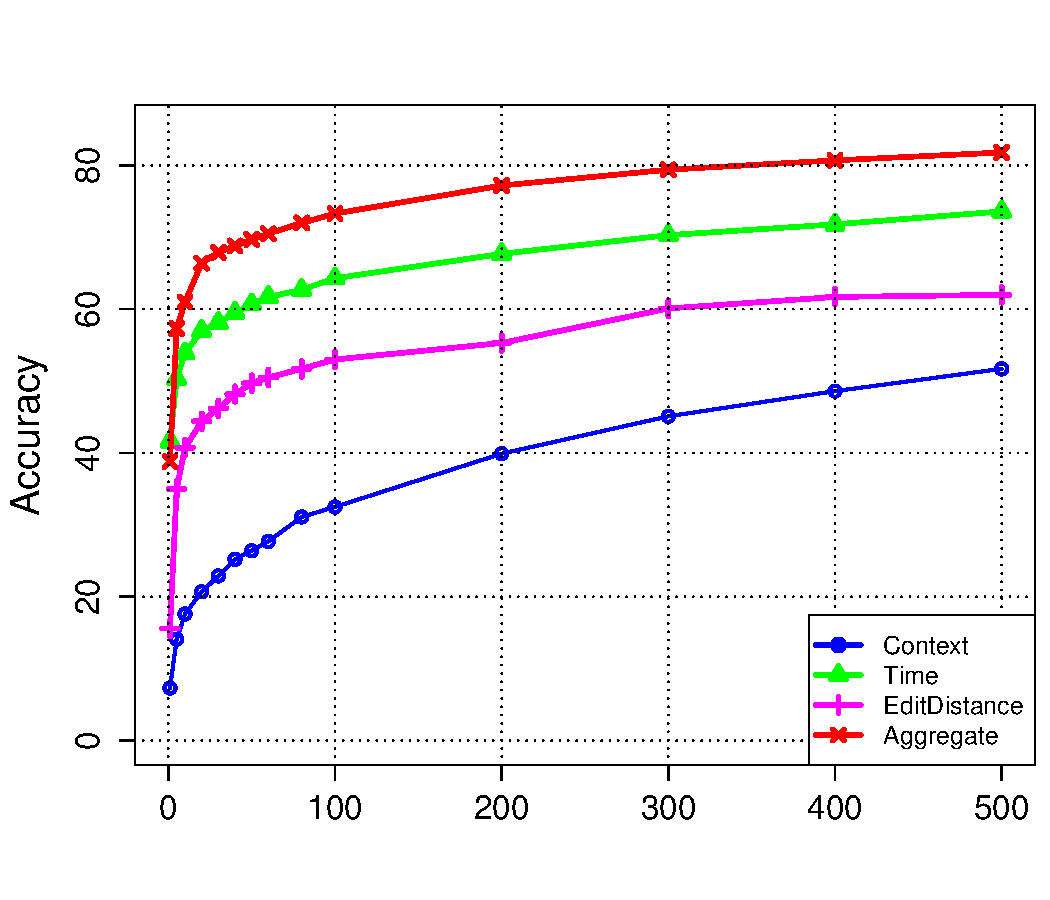
\includegraphics[width=2.4in]{figures/exp1/parallel.freq/parfreq} 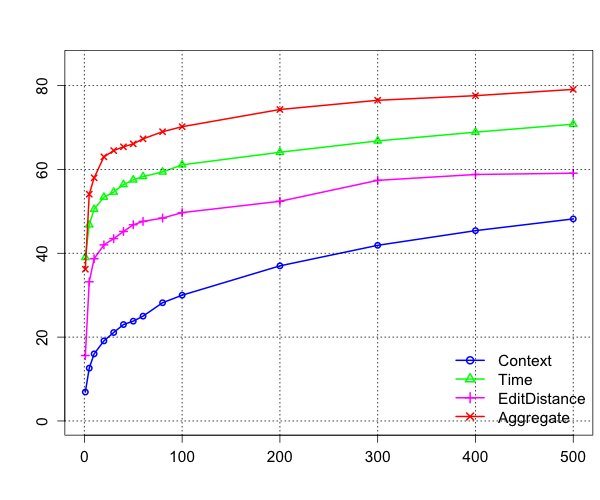
\includegraphics[width=2.4in]{figures/exp1/parallel.rand/parrand}}}
\centerline{\mbox{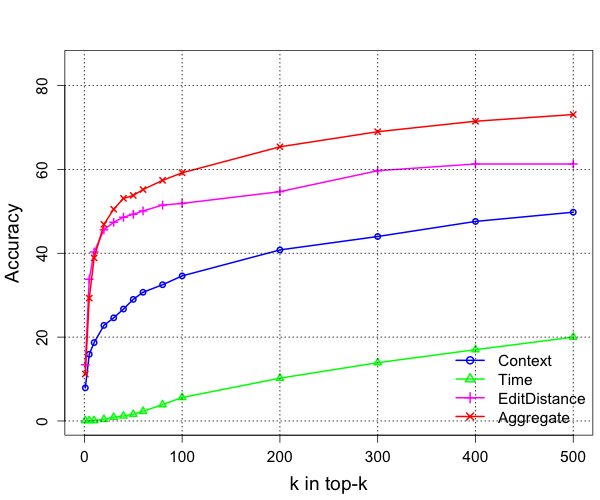
\includegraphics[width=2.4in]{figures/exp1/wikinews.freq/wikinewsfreq} 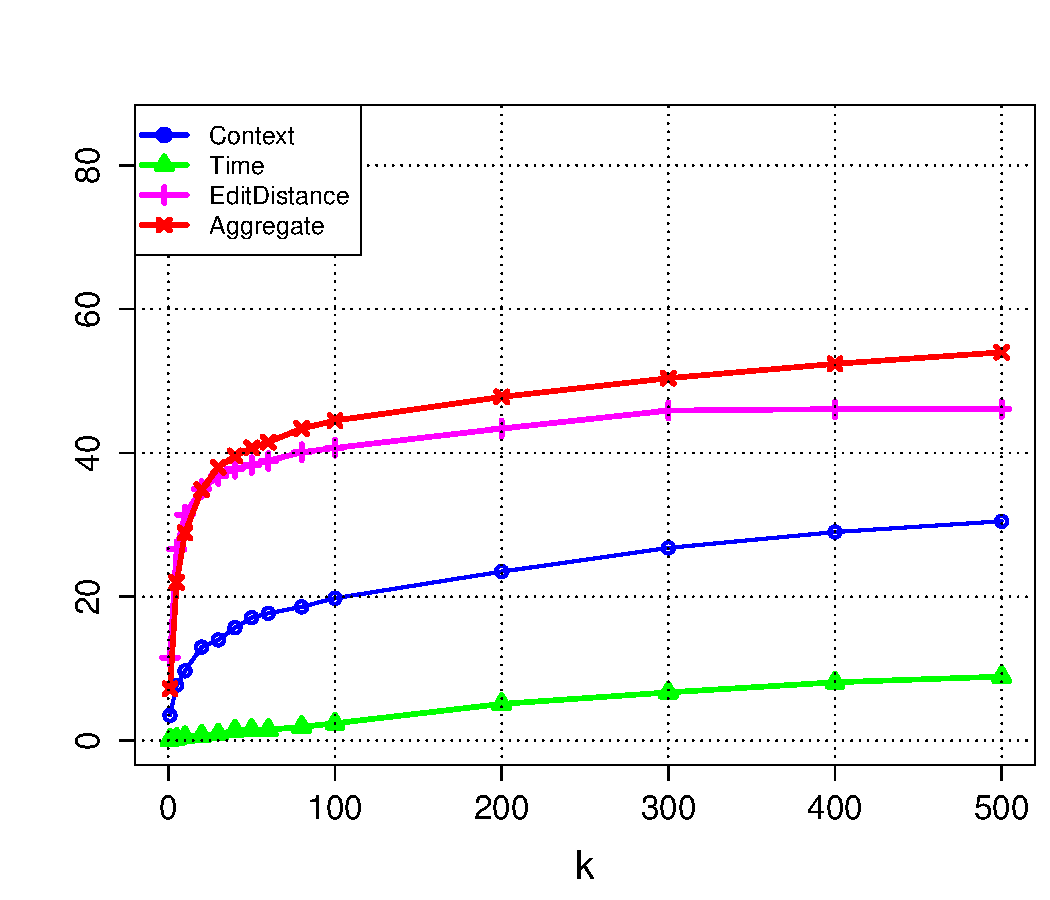
\includegraphics[width=2.4in]{figures/exp1/wikinews.rand/wikinewsrand}}}
\caption{Accuracy on parallel en-es data for most frequent (top left) and random (top right) 1000 source words, and on wikipedia / newswire for most frequent (bottom left) and random (bottom right) 1000 source words.}
\label{fig:exp1}
\end{figure}

We repeat the same experiment using wikipedia and newswire data to derive dictionaries from contextual and temporal cues, respectively (\figref{fig:exp1}, bottom).  Since the newswire corpora is only weakly temporally aligned, the performance of the temporal cue drops substantially.  Still, the cues provide informative and non-redundant signals, which can be combined to obtain better quality lexicons.  Notice the substantial drop in performance (about {\bf 19\%}) for randomly selected source tokens.  While not entirely surprising, it supports our observation that evaluating on frequent source words alone can be misleading if the objective is to induce wide coverage dictionaries.\\

\begin{table}[h!]
\setlength{\tabcolsep}{1ex}
\footnotesize
\begin{center}
\begin{tabular}{lllll}
\multicolumn{3}{c}{cues}\\
\cline{1-3}
contextual		&	temporal	&	orthographic	&	MRR	\\
\hline
sadam	&	{\bf autoritario}	&	{\em autoritaria}, {\em autoritarias} &	{\bf autoritario}	\\
{\bf autoritario}	&	democracia	&	{\bf autoritario}, {\em autoritarios} &	sadam\\
az\'{u}car	&	{\em autoritarios}	&	autoritarismo, \dots &	{\em autoritaria}\\
perfeccionamiento	&	país	&	 autorizadas, \dots &	{\em autoritarias}\\
tr\'{a}nsito	&	democr\'{a}ticas	&	horarias, \dots &	{\em autoritarios}\\
apartheid	&	elecciones	&	autocar comisaria \dots &	democracia\\
transitorio	&	fuerzas	&	&	az\'{u}car\\
totalitario	&	vecino	&	&	perfeccionamiento, país\\
talib\'{a}n	&	democr\'{a}ticos	&	&	democr\'{a}ticas, tr\'{a}nsito\\
dictatorial	&	{\em autoritaria}	&	&	elecciones, apartheid\\
\hline
{\bf infantil}	&	{\em lactantes}	&	{\bf infantil}, infame, \dots &	{\bf infantil}\\
materna	&	mortalidad	&	infames, infamia, \dots &	{\em lactantes}\\
maternal	&	sociedad	&	isaf, influir, \dots &	materna, mortalidad, \dots\\
morbilidad	&	nivel	&	&	maternal, sociedad\\
índice	&	problema	&	&	morbilidad, nivel\\
tasa	&	trabajo	&	&	índice, problema\\
disminuiría	&	países	&	&	tasa, trabajo\\
cr\'{o}nico	&	tiempo	&	&	países, disminuiría\\
escape	&	reducci\'{o}n	&	&	 cr\'{o}nico, tiempo\\
derivada	&	desarrollo	&	&	reducci\'{o}n, escape\\
\hline
{\bf almacenamiento}	&	{\bf almacenamiento}	&	jorge, seora, \dots	&	{\bf almacenamiento}\\
{\bf almacenaje}	&	nuclear	&	saturado, gestoras, \dots	&	{\bf almacenaje}, nuclear\\
recoger	&	radiactivos	&	&	recoger, radiactivos\\
m\'{e}dico	&	almacenar	&	&	almacenar, m\'{e}dico\\
tratamiento	&	radioactivos	&	&	tratamiento, radioactivos\\
servicio	&	propuesta	&	&	propuesta, servicio\\
viaje	&	normas	&	&	viaje, normas\\
vuelo	&	peligro	&	&	vuelo, peligro\\
registro	&	llegar	&	&	llegar, registro\\
etc	&	instalaciones	&	&	instalaciones, etc\\
\end{tabular}
\end{center}
\normalsize
\caption{Top ranked translations for {\bf authoritarian}, {\bf infant}, {\bf storage} (top, middle, bottom, respectively) inferred from context, temporal, and orthographic cues and aggregated with the MRR heuristic.  Correct translations are in bold if found in the test dictionary and italicized otherwise.}
\label{fig:examplelists}
\end{table}

\tabref{fig:examplelists} contains ranked lists of translations induced from the three cues and aggregated using the MRR heuristic for three sample english words: authoritarian, infant, and storage.  Note the numerous morphological variants of the correct translations and alternative translations not found in the dictionary (italicized).  Also notice that when some signals are not informative (e.g. the orthographic cue in the third example) others may still be sufficient to induce the correct candidates at the top of the aggregated list.

\subsection{Context vs.\ alignments} 

Word alignments can be induced directly from sentence aligned corpora.  In this set of experiments, we compare bilingual lexicons derived from word alignments (produced by GIZA++, \cite{Och:2003}) to those generated from the contextual cue alone on the English-Spanish section of the Europarl corpus (see \figref{fig:exp2}). While word alignments induce a much more informative signal than context alone, sufficient sentence aligned bilingual data is not available for most of the low resource languages we consider in this work.\\

\begin{figure}[h!]
\centerline{\mbox{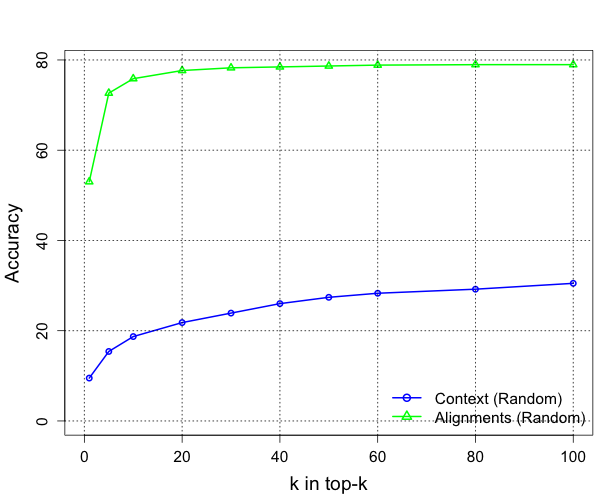
\includegraphics[width=3in]{figures/exp2/alignvscontext}}}
\caption{Accuracy of lexicons induced from alignments and context on parallel en-es data for random 1000 source words.}
\label{fig:exp2}
\end{figure}

\subsection{Lexicon induction for a low-resource languages}

Next, we selected 10 low resource languages for which we have collected sufficient amount of newswire data and have seed dictionaries in an appropriate script: Welsh, Farsi, Indonesian, Latvian, Russian, Slovak, Albanian, Serbian, Turkish, and Uzbek.  \figref{fig:exp3} shows the accuracy of lexicons induced from the contextual (top), and temporal (middle) cues, and the MRR aggregation scheme (bottom); results for 1000 most frequent and random source words are shown on the left and right, respectively.\\

Similarly to the experiments in \secref{sect:exphigh}, lexicon accuracy drops on random source words for Russian and Turkish.  For the remaining languages, low dictionary coverage means a large overlap between 1000 random and most frequent test dictionary terms.  That is, both sets of experiments effectively test the accuracy on random source words, since test dictionary entries themselves were selected at random. \mtodo{Confusing? Drop most frequent?}  Both temporal and contextual cues are informative, but the simple aggregation heuristic fails to provide an improvement.  While simple ensemble schemes typically work well for a large number of diverse signals, a more sophisticated approach to combining few available ranked lists remains the subject of our ongoing work.\\

\begin{figure}[h!]
\centerline{\mbox{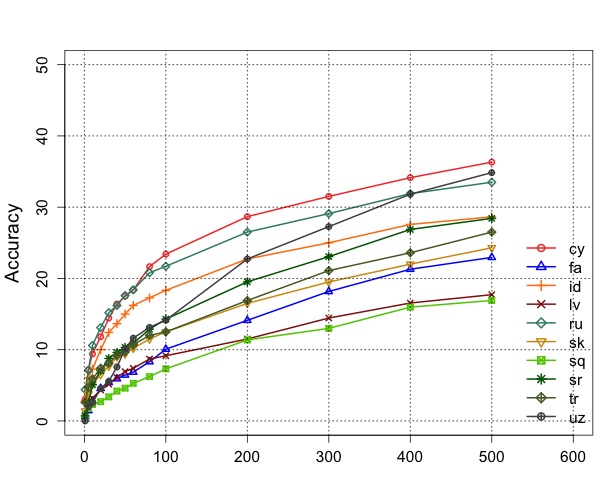
\includegraphics[width=2.4in]{figures/exp3/freq/freqcontext} 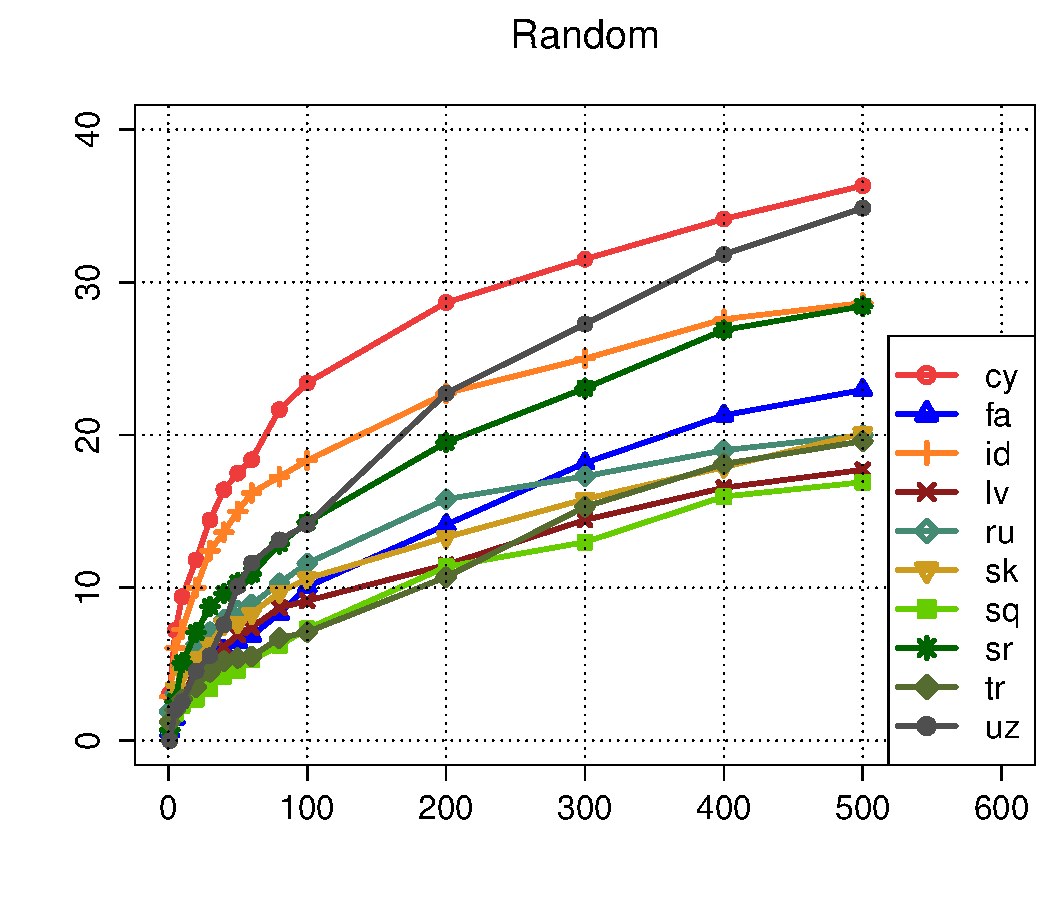
\includegraphics[width=2.4in]{figures/exp3/rand/randcontext}}}
\centerline{\mbox{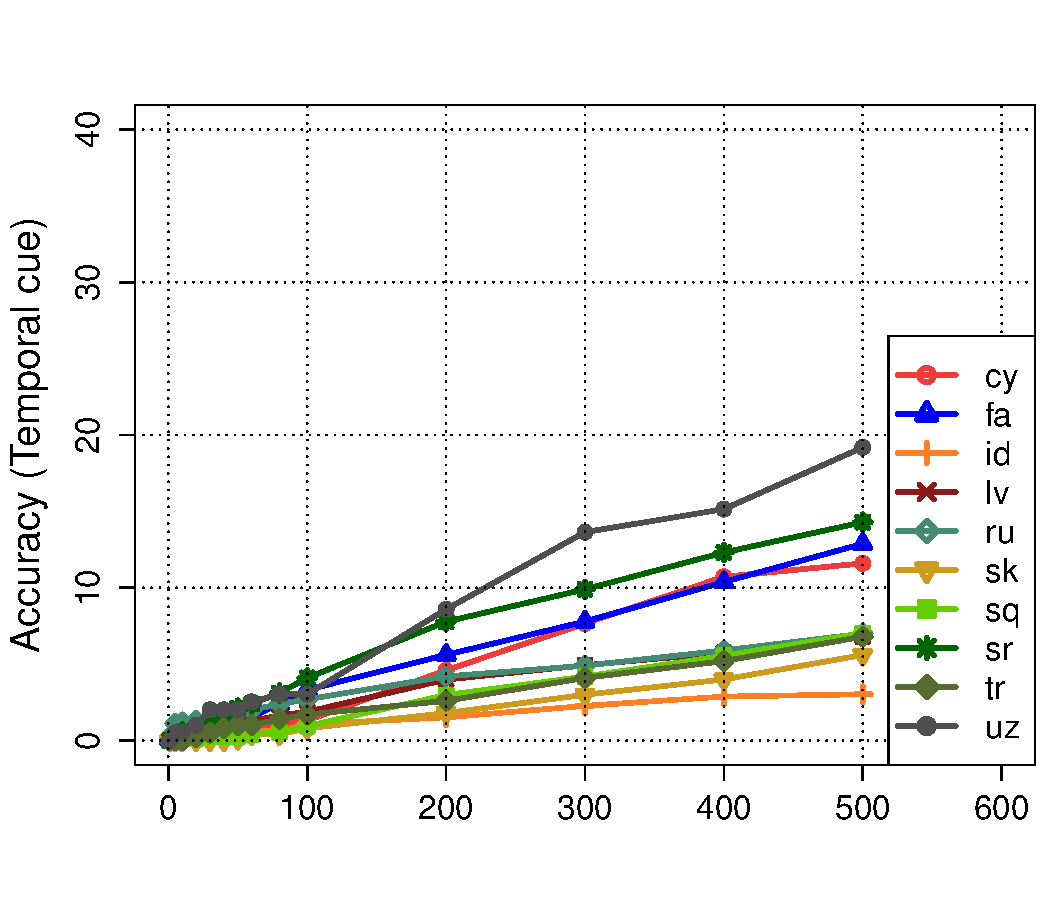
\includegraphics[width=2.4in]{figures/exp3/freq/freqtime} 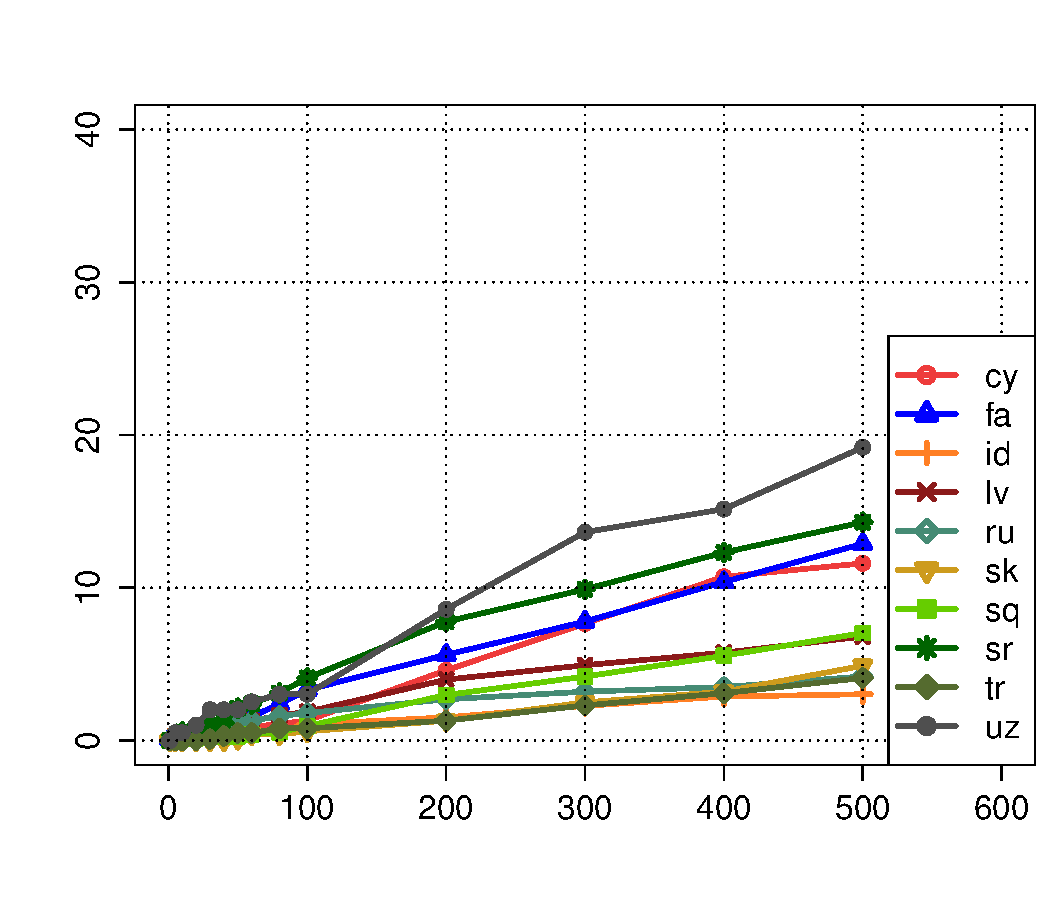
\includegraphics[width=2.4in]{figures/exp3/rand/randtime}}}
\centerline{\mbox{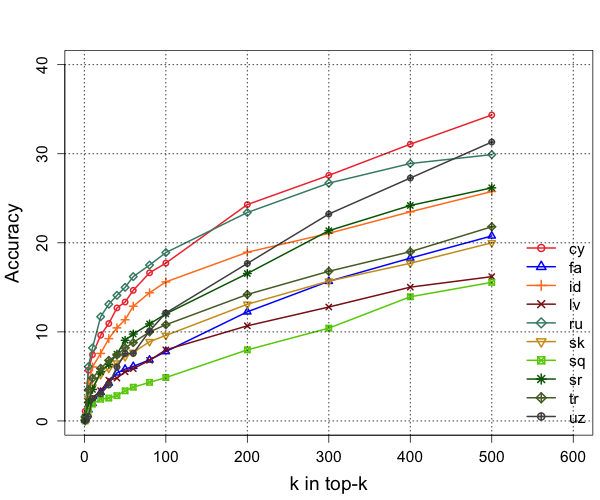
\includegraphics[width=2.4in]{figures/exp3/freq/freqmrr} 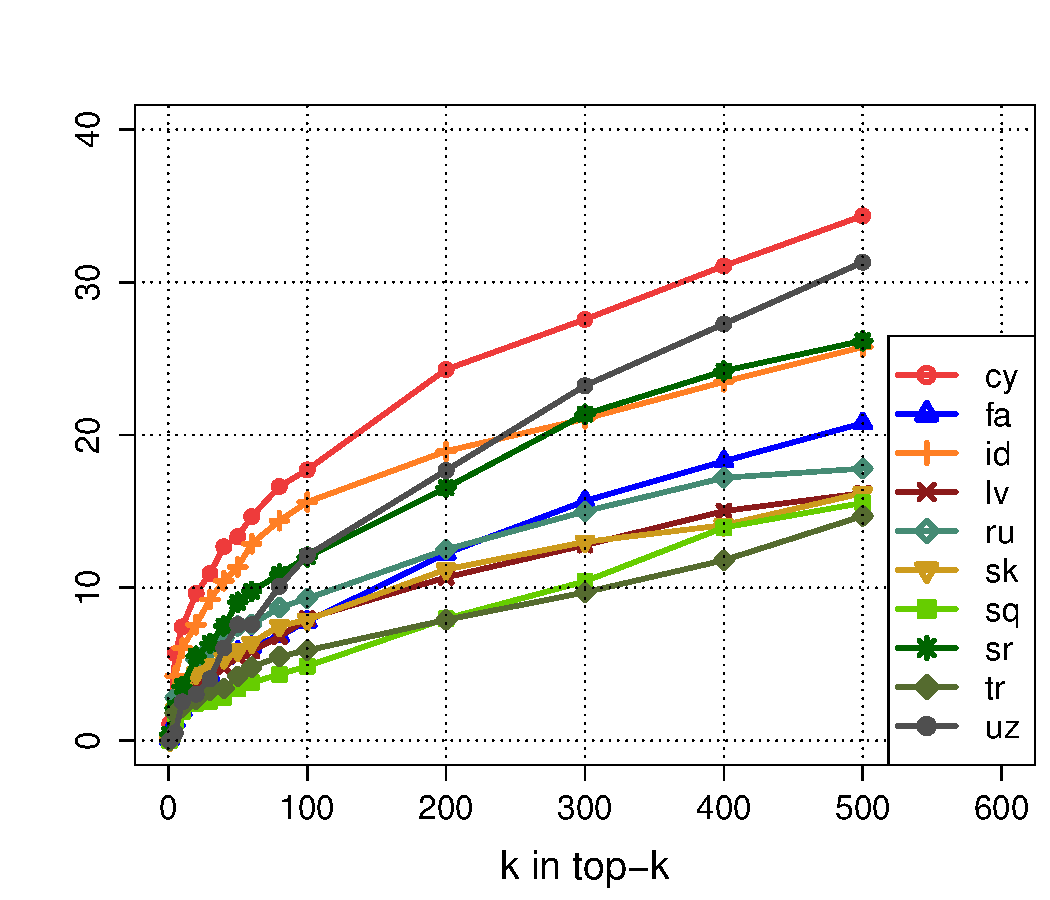
\includegraphics[width=2.4in]{figures/exp3/rand/randmrr}}}
\caption{Accuracy of contextual (top) and temporal (middle) cues and the MRR scheme (bottom) for most frequent (left) and random (right) 1000 source words for Welsh (cy), Farsi (fa), Indonesian (id), Latvian (lv), Russian (ru), Slovak (sk), Albanian (sq), Serbian (sr), Turkish (tr), and Uzbek (uz).}
\label{fig:exp3}
\end{figure}

\subsection{Crowd-sourcing annotation} \label{sect:mturk}

We use our existing bilingual dictionaries to induce large bilingual lexicons via the contextual cue and to evaluate their accuracy.  However, these dictionaries vary substantially in quality and coverage across languages and corpora (see \secref{sect:resources}).  In this set of experiments we follow previous work on crowd-sourcing annotations \cite{Snow:2008,CCB:2009} and study \cite{Irvine:2010} the viability of obtaining translations for a low-resource languages specifically for use in our induction framework.  First, we use the contextual cue to induce lexical translation pairs from the Wikipedia monolingual data. Then, we pay Amazon Mechanical Turk (MTurk) workers a small amount to check and correct our system output. We can then use the updated lexicons to inform another iteration of lexicon induction, gather a second set of MTurk annotations, and so on. \\

For 32 of the 42 languages in \tabref{fig:wikidictstats}, we were able to induce lexical translation candidates and post them on MTurk for annotation. For these languages we presented annotators with top ten scored candidates for a set of 100 English words and asked them to mark correct translations. If our seed dictionary included an entry for a source word, we included the translation in the candidate list as a positive control. Additionally, we included a random word in the foreign language as a negative control.  We do not have dictionaries for the remaining 10 languages, so we asked workers to type translations for 100 English words. We had three distinct workers provide such annotations for each source word. \\ 

\begin{figure}[h!]
\centerline{\mbox{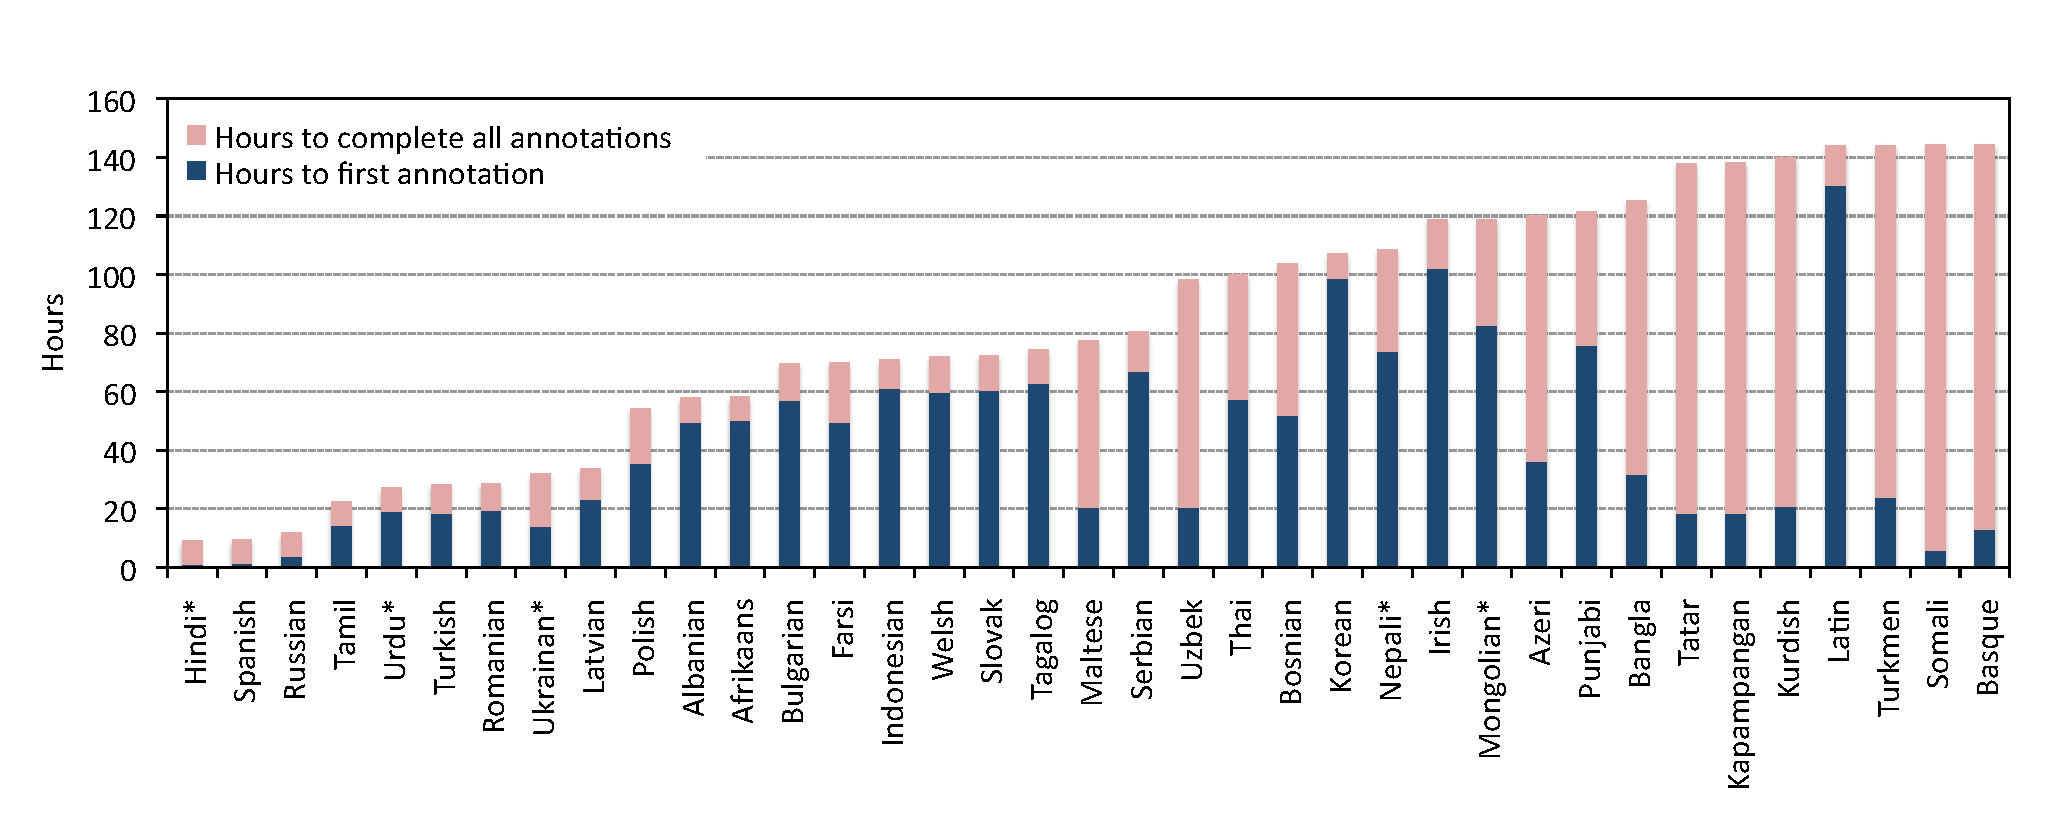
\includegraphics[width=5in]{figures/exp4/time}}}
\centerline{\mbox{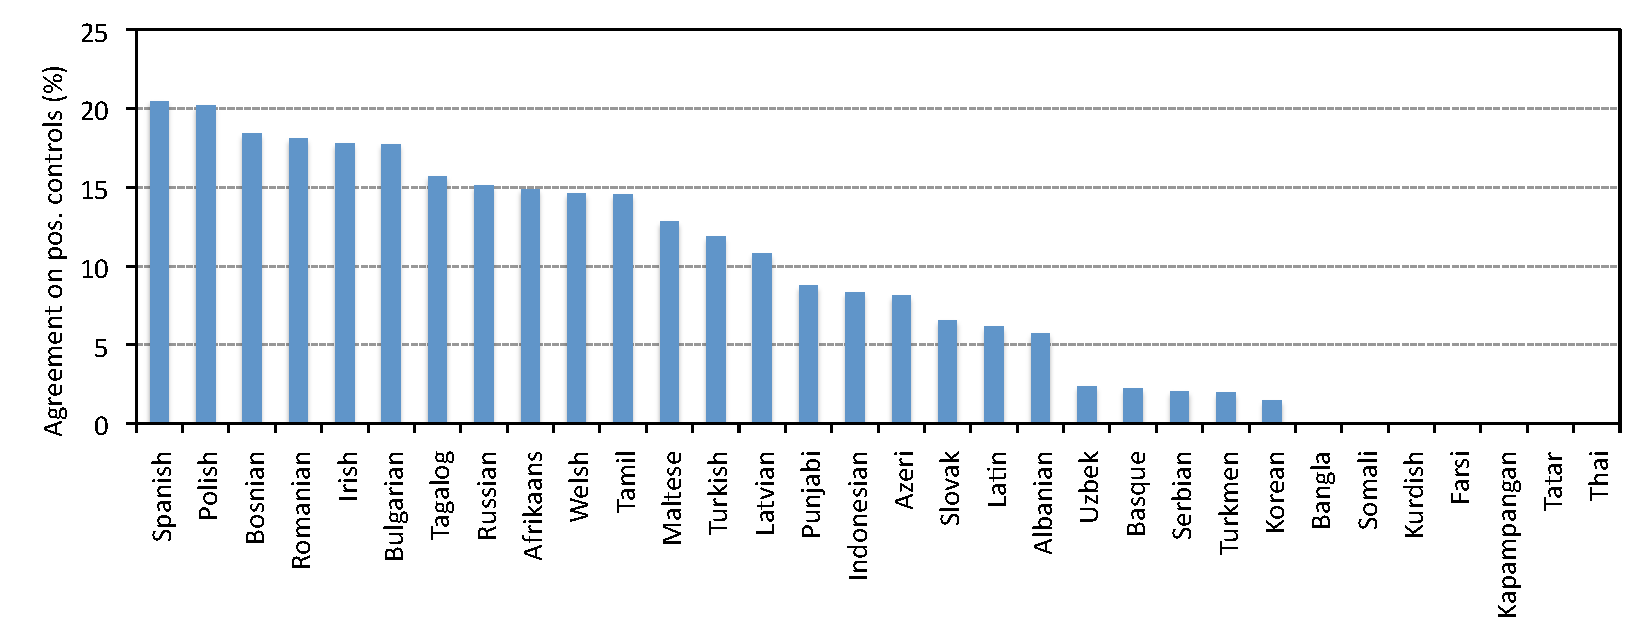
\includegraphics[width=5in]{figures/exp4/controls}}}
\caption{Top: time to complete annotation of 100 English words.  Division of the time between posting and the completion of the first annotation unit (HIT) and the time between the completion of the first and last HIT shown. HITs that required lexical translation only are marked with an $*$. Bottom: percent of positive control candidate translations for which two or three workers checked as accurate.}
\label{fig:exp4}
\end{figure}

\figref{fig:exp4} (top) shows the time it took to complete annotation of for 37 languages on MTurk. Annotations the following languages were posted for a week and were never completed: Tigrinya, Uighur, Tibetan, Kyrgyz, and Kazakh. All five of the uncompleted required typing annotations, a more time consuming task than checking translation candidates. Not surprisingly, languages with many speakers (Hindi, Spanish, and Russian) and languages spoken in and near India (Hindi, Tamil, Urdu) were completed very quickly. \figref{fig:exp4} (bottom) shows the percent of positive control candidate translations that were checked by the majority of workers (at least two of three). The highest amounts of agreement with the controls were for Spanish and Polish, which indicates that those workers completed the annotations more accurately than the workers who completed, for example, the Tatar and Thai annotations. However, the seed dictionaries are very noisy, so this finding may be confounded by discrepancies in the quality of our dictionaries. The noisy dictionaries also explain why agreement with the positive controls is, in general, relatively low.\\

To understand the utility of MTurk generated translation for inducing lexicons, we supplemented our dictionaries for each of the 37 languages for which we gathered MTurk annotations with translation pairs that workers agreed were good (both chosen from the candidate set and manually translated). We compared seed dictionaries of size 200 with those supplemented with, on average, 69 translation pairs. We found an average relative increase in accuracy of our output candidate set (evaluated against complete available dictionaries) of {\bf 53\%}.\\

In sum, we found that the iterative approach of automatically generating noisy annotation and asking MTurk users to correct it to be an effective means of obtaining supervision.  These correction tasks are simple, can be completed quickly for a large number of low resource languages, and produce high quality annotation.

%-----------------------------------------------------
\section{System Overview}

In this section we touch on some of the implementation details of the lexicon induction framework: we overview the data collection and lexicon induction procedures and explain how the framework can be extended to include new monolingual resources and cues derived from them.  

\subsection{Data Collection} \label{sect:datacollect}

While some monolingual resources (see \secref{sect:resources}) are static, others require ongoing collection.  We have set up the nutch crawler\footnote{http://nutch.apache.org/} to continuously crawl a number of web sites generating news content in the languages of interest.  The crawl results are periodically processed (see \figref{fig:data}) to (1) parse page content and extract metadata associated with the page, (2) merge with previously extracted pages, (3) identify language of the page content, and (4) generate time annotated corpora for each of the languages.  See \tabref{fig:wikidictstats} for a current summary of the collected data.

\begin{figure}[h]
\centerline{\mbox{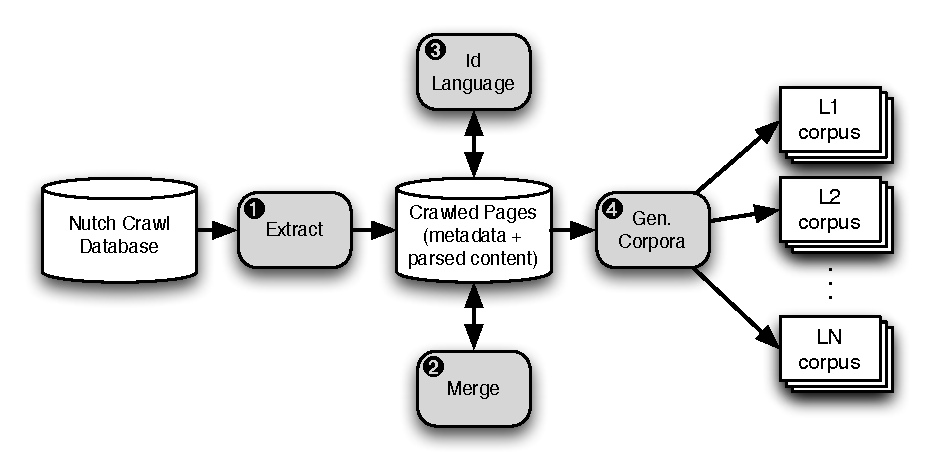
\includegraphics[width=3in]{figures/datacollect}}}
\caption{Ongoing data collection.}
\label{fig:data}
\end{figure}

\subsection{Lexicon Induction Procedure}

Let us turn to the induction procedure, highlight some of the most relevant code, and show how the framework can be extended to include new monolingual resources and cues.  \figref{fig:packages} shows the implementation layout and \figref{fig:system} gives a high level view of the lexicon induction procedure.\\

\begin{figure}[h]
\centerline{\mbox{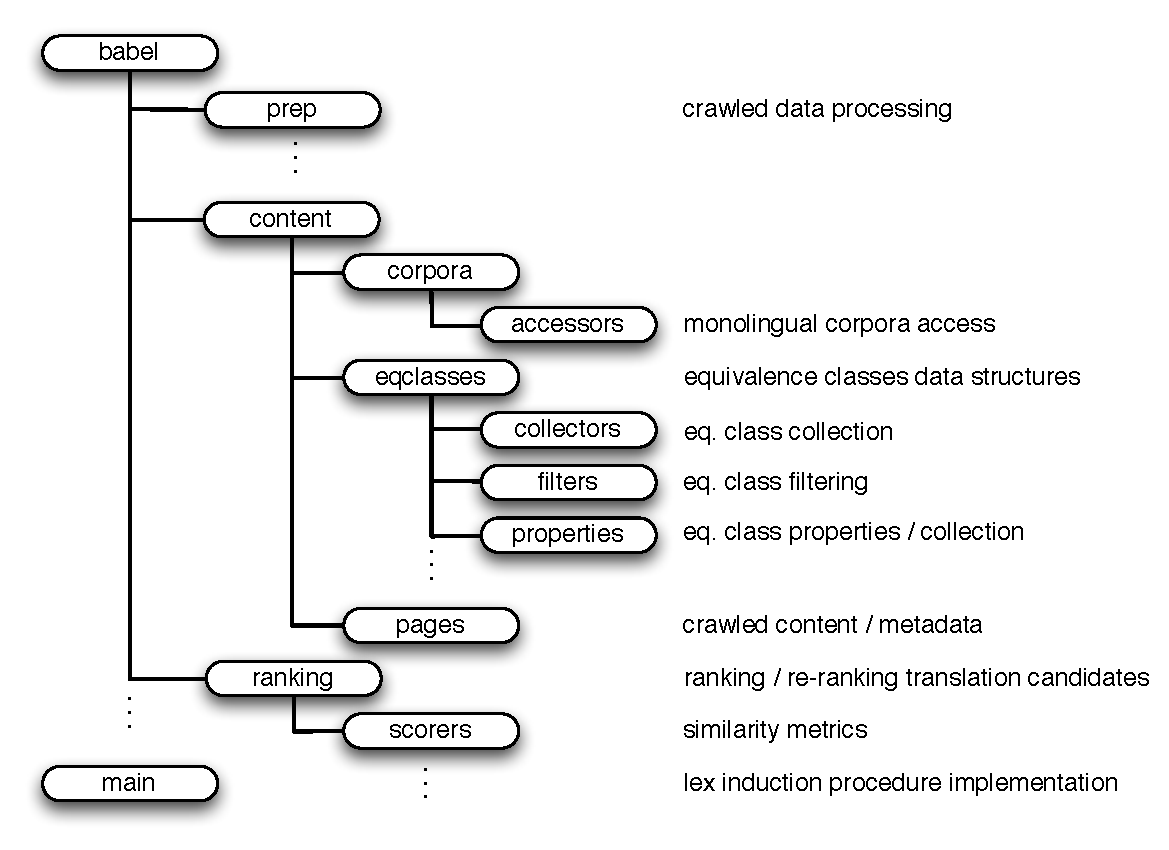
\includegraphics[width=3in]{figures/packages}}}
\caption{Package layout of the lexicon induction framework.}
\label{fig:packages}
\end{figure}

We argued in \secref{sect:morph} that collecting aggregate statistics for morphological variants of a single lexeme is important when dealing with morphologically rich languages.   Base class \small{\tt EquivalenceClass} groups morphological variants present in the data into equivalence classes and maintains a set of aggregate statistics derived from monolingual cues.  In turn, each of the statistics, or properties, is implemented by a subclass of \small{\tt Property}. \\

\begin{figure}[h!]
\centerline{\mbox{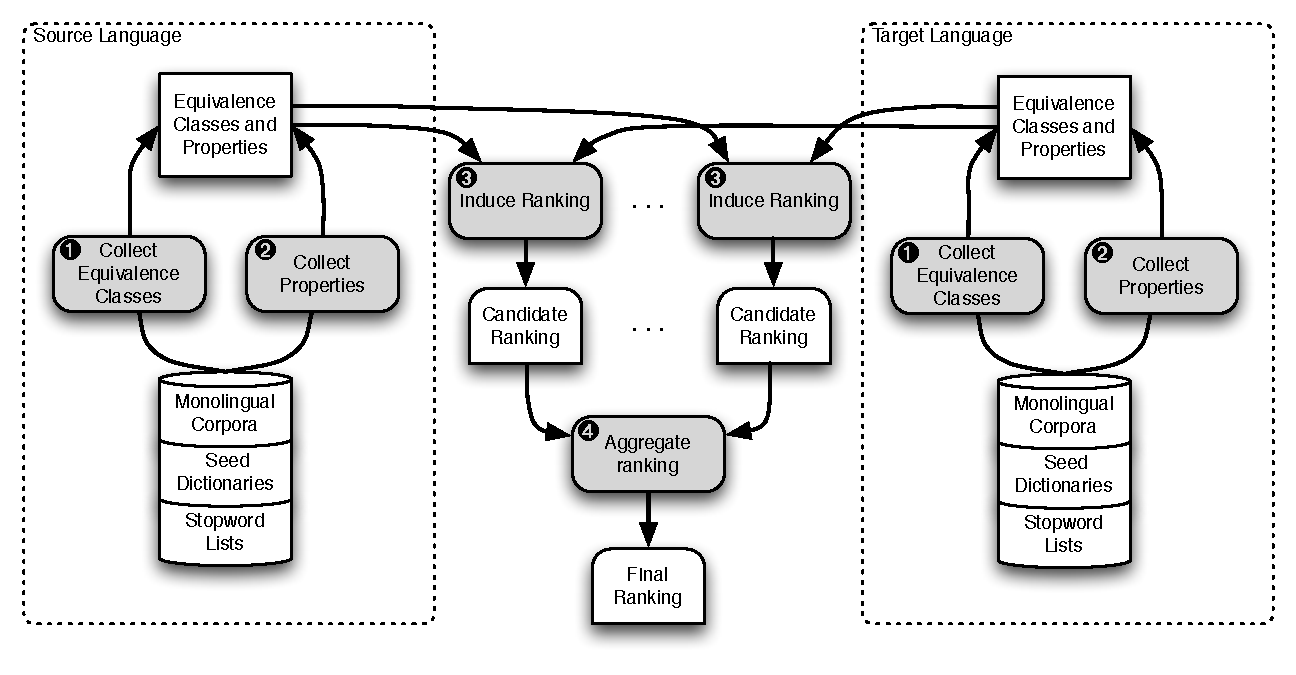
\includegraphics[width=4in]{figures/lexinduct}}}
\caption{A high level overview of the lexicon induction framework.  Equivalence classes and corresponding properties are first extracted from monolingual data (steps 1 and 2).  Similarity metrics defined over the properties are then used top produce rankings over target candidates in step 3.  Finally, ranked lists are aggregated to produce the final rankings in step 4.}
\label{fig:system}
\end{figure}

The induction procedure begins with two passes through both source and target language monolingual corpora (step 1 and 2 on \figref{fig:system}, respectively) implemented in \small{\tt DataPreparer}.  Each of the available corpora (e.g. see \secref{sect:resources}) is accessed through a corresponding subclass of \small{\tt CorpusAccessor}.  In the first pass, morphological variants are collected (see \small{\tt EquivalenceClassCollector}) to generate the corresponding equivalence classes and, in the second pass, a set of properties such as contextual vectors, temporal distributions, topic information, etc.\ is collected for each of the equivalence classes. The initial set of equivalence classes is pruned by a series of filters extending \small{\tt EquivalenceClassFilter} in order to throw out patently incorrect or undesirable candidates, e.g. stop words, least or most frequent classes, strings containing numbers or letters of a wrong script, etc. Both source and target equivalence classes along with the collected statistics are persisted on disk.\\

Next, collected properties along with the corresponding similarity metrics extending \small{\tt Scorer} are used to produce a ranked list of candidates for each of the source equivalence classes.  This step involves a substantial amount of computation since each of the source equivalence classes is compared with all of the target candidates. Its implementation in \small{\tt Ranker} is parallelized, which substantially speeds up this step.  Ranked candidate lists induced for each source equivalence class from multiple cues are aggregated (see \small{\tt Reranker}) into a joint ranking in step 4 on \figref{fig:system}  Finally, the induced ranked candidate lists are evaluated in \small{\tt NBestCollector}.\\

\lstref{fig:cfg} shows an example configuration file for setting up the induction process.  It is split into 5 sections, one would:

\begin{itemize}
  \item The \small{\tt  corpora} section lists both source and target monolingual corpora with additional configuration parameters specific to the corresponding subclass of \small{\tt CorpusAccessor}.
  \item The \small{\tt  resources} section specifies additional resources, such as stop word lists and bilingual dictionaries.
  \item The \small{\tt  preprocessing} section configures the two stage preprocessing stage, i.e. which resources to use to generate equivalence classes and how to collect their properties.  For example, the \small{\tt  candidates} section on \lstref{fig:cfg} specifies that the simple and prefix heuristics (see \secref{sect:morph}) should be used for generating source and target equivalence classes, respectively, and that the classes should be pruned if they occur fewer than 10 times in the data.
  \item Finally, the \small{\tt experiments} section configures the induction process.  The configuration parameters can be used to choose most frequent or random source equivalence classes for induction (\small{\tt RandomSource}), the portion of the dictionary to use for projecting contextual vectors (\small{\tt DictionaryPercentToUse}), the target candidate ranked lists size to induce  (\small{\tt NumTranslationsToAddPerSource}), the number of threads to use when generating rankings (\small{\tt NumRankingThreads}), and to specify which properties are to be used to induce those rankings and whether or not to aggregate them (\small{\tt DoAggregate}).\\
\end{itemize}

In order to extend the framework to add a new monolingual resource and/or include additional cues:

\begin{itemize}
  \item Extend \small{\tt CorpusAccessor} to enable access to a new resource.
  \item Extend \small{\tt Property} and \small{\tt PropertyCollector} to manage and collect desired statistics from a monolingual resource.
  \item Extend \small{\tt Scorer} to implement a similarity metric for scoring a source and a target candidate equivalence classes.
\end{itemize}

%\newpage
\lstinputlisting[caption=Example configuration file.,label=fig:cfg]{figures/babel.xml}
%\newpage

%-----------------------------------------------------
\section{Conclusions and Future Work}

\begin{itemize}
  \item Investigated the efficacy of monolingual cues for a number of low-density languages / resources. If the objective is wide coverage, results reported in prior work are misleading.
  \item Bilingual lexicons is preliminary step for low resource MT.  Incorporate metric scores as features.
  \item Aggregation schemes for few signals and some amount of supervised data.
\end{itemize}

%-----------------------------------------------------
% Notes: 
% *  Select most freq. words from the entire dictionary not just test.
% *  Never tried using the entire wiki (not just the interlinked pages) and newswire data for also gathering contexts.
%-----------------------------------------------------

\bibliographystyle{apalike}
\bibliography{references}
 
\end{document}
